\documentclass[11pt]{article}
\usepackage[a4paper,margin=2.5cm]{geometry}
\usepackage[T1]{fontenc}
\usepackage{lmodern}
\usepackage{microtype}
\usepackage{amsmath,amssymb}
\usepackage{graphicx}
\usepackage{booktabs}
\usepackage{xcolor}
\usepackage[hidelinks]{hyperref}
\usepackage[numbers,sort&compress]{natbib}
\usepackage{caption}
\setlength{\emergencystretch}{3em}
\captionsetup{font=small,labelfont=bf}

\newcommand{\bmc}{\textsc{bmc}}

\title{Train Less, Contribute More:\\A Neural-Architecture Search for Numerai's Ender Target}
\author{Volodymyr Borysenko\\\small University of California, Berkeley}
\date{October 2026}

\begin{document}
\maketitle

\begin{abstract}
We search for the neural network that best predicts Numerai's 20-day Ender target, judging
models not by raw correlation but by benchmark model contribution (\bmc{}): the signal a model
adds beyond Numerai's own LightGBM benchmark. Across 35 cross-validated runs in six rounds we
compare plain, wide, deep and residual multilayer perceptrons (MLPs), a TabM-style
BatchEnsemble, learned per-bin feature embeddings, two loss functions and the main training
hyperparameters. The best model is a plain three-layer MLP (1024--512--256) trained with a
per-era Pearson-correlation loss for a short time. Averaged over three seeds it reaches
\bmc{}~0.0089 over the last 200 out-of-fold eras, $2.1\times$ a LightGBM baseline trained on
the same data. Architecture mattered far less than one variable: the amount of training.
Training moves predictions steadily away from the benchmark, raising \bmc{}, until it starts
to destroy raw signal; every knob we varied (epochs, learning rate, batch size, dropout) lands
on this single curve. On 613 eras never used during the search, the result transfers once the
training amount is held fixed in optimizer steps rather than epochs: the 6-epoch recipe
over-trains on twice the data, while 4~epochs recovers \bmc{}~0.0082. This matches the
continuous-time view of early stopping as ridge regularization.
\end{abstract}

\section{Introduction}

Numerai runs a stock-market prediction tournament on obfuscated data: each week (an
\emph{era}) participants rank several thousand stocks from a few thousand anonymized
features, and are paid for predictions that improve Numerai's meta model. A model with high
raw correlation that merely re-discovers what Numerai's benchmark models already know
contributes little. Benchmark model contribution (\bmc{}) measures this directly as the
correlation of a model's predictions with the target after neutralizing them against the
benchmark's predictions \citep{forum_benchmark_models,numerai_scoring}.

Gradient-boosted trees dominate tabular prediction \citep{grinsztajn2022tree}, and the
tournament's benchmark is itself a LightGBM model. Neural networks therefore have a natural
advantage for \bmc{}: their inductive bias differs from that of trees, so even at lower raw
correlation they may carry more \emph{unique} signal. This paper asks which neural
architecture, loss and training recipe maximize that unique signal.

Our contributions are:
\begin{enumerate}
  \item A controlled architecture search, one variable at a time with seed-averaged
        confirmation, showing that a plain MLP beats residual, ensemble and embedding-based
        alternatives on \bmc{}.
  \item Evidence that \bmc{} is governed by the \emph{amount} of training, and that this
        trade-off has a single interior optimum shared by all training knobs.
  \item A confirmation on disjoint data showing that the optimum is a fixed number of
        optimizer steps, so the epoch count must shrink as the training set grows.
\end{enumerate}

\section{Related work}

\paragraph{Machine learning for cross-sectional returns.}
Neural networks and trees improve out-of-sample return prediction over linear models through
nonlinear interactions, and shallow networks outperform deeper ones \citep{gu2020empirical};
later work learns factor structure \citep{gu2021autoencoder} or a stochastic discount factor
with moment-based losses \citep{chen2024deep}, and finds machine-learning profits concentrated
in hard-to-arbitrage stocks \citep{avramov2023machine}. Whether model complexity is a virtue
\citep{kelly2024virtue} remains debated \citep{nagel2025seemingly,fallahgoul2025high}.
Losses closer to the trading objective, such as ranking \citep{poh2020building,lin2026lambdarankic},
classification \citep{bai2021classification}, Sharpe-ratio \citep{zhang2020deep} and
correlation losses \citep{forum_custom_loss}, often beat squared error. Hedging unpriced risk
\citep{daniel2020cross} motivates the feature neutralization common on Numerai
\citep{forum_neutralization_intro,forum_neutralization_bias}; forecast combination
\citep{rapach2010out}, auxiliary targets \citep{forum_new_targets}, dynamic ensembling under
regime change \citep{wong2023online} and era boosting \citep{forum_era_boosting} are other
recurring tools. Repeated configuration search inflates backtests
\citep{bailey2014deflated,bailey2017probability,arian2024backtest}; shrinkage is a classic
remedy \citep{kozak2020shrinking}.

\paragraph{Tabular deep learning.}
Recent work revisits MLP, ResNet and transformer baselines \citep{gorishniy2021revisiting},
numerical feature embeddings \citep{gorishniy2022embeddings}, parameter-efficient ensembles
\citep{gorishniy2025tabm}, well-tuned default MLPs \citep{holzmuller2024better} and heavily
regularized plain networks \citep{kadra2021well}. Attention-based models \citep{somepalli2021saint}
and tabular foundation models \citep{hollmann2025tabpfn,tabpfn25,tabpfn3} do not yet scale to
millions of rows with hundreds of features. Weight averaging \citep{izmailov2018averaging},
deep ensembles \citep{lakshminarayanan2017simple} and model soups \citep{wortsman2022model}
reduce variance.

\paragraph{Training dynamics and differential equations.}
Gradient flow stopped at time $t$ behaves like ridge regression with penalty $\lambda = 1/t$
\citep{ali2019continuous}; finite learning rates add an implicit gradient penalty whose
strength scales with the learning rate and, for stochastic gradients, inversely with batch
size \citep{barrett2021implicit,smith2021origin,li2017stochastic}. Decay towards the
initialization is the explicit counterpart of early stopping \citep{li2018explicit}, and noise
injection acts as Tikhonov or heat-equation smoothing
\citep{bishop1995training,camuto2020explicit,campbell2020deterministic,wang2024convection}.
Continuous-depth networks
\citep{chen2018neural,dupont2019augmented,finlay2020train,kelly2020learning,haber2017stable,ruthotto2020deep}
and their stochastic and controlled variants
\citep{liu2019neural,li2020scalable,kidger2020neural} have been applied to finance
\citep{gierjatowicz2020robust,yang2021neural}, building on stochastic-calculus models of
prices \citep{black1973pricing}, but we found no application to static cross-sectional
ranking.

\paragraph{Number theory.}
Its one documented use relevant here is quasi-Monte Carlo search: low-discrepancy sequences
cover a hyperparameter space more evenly than random draws
\citep{bousquet2017critical,roy2023qmc}. Random Fourier features
\citep{rahimi2007random,avron2016qmc} and feature hashing \citep{weinberger2009feature} are
related tools that do not fit dense, low-cardinality features.

\section{Experimental setup}

\paragraph{Data.} Numerai v5.3, \texttt{medium} feature set (780 features, each an integer bin
$0$--$4$), target \path{target_ender_20}. Because experiments ran on a 16\,GB laptop, the
search used every fourth era of the training and validation data (307 eras, 1.7M rows;
\emph{scout data}). The confirmation step used every second era at offset one (613 eras, 3.4M
rows; \emph{scale data}), which shares no eras with the scout data.

\paragraph{Validation.} Five expanding-window folds over eras with a 13-era embargo. The first
fold has no training data, so out-of-fold (OOF) predictions cover the last four folds. Every
network trains for a fixed number of epochs; there is no early stopping, so no validation
information leaks into OOF scores.

\paragraph{Metrics.} The primary metric is mean \bmc{} over the last 200 OOF eras against the
official \path{v53_lgbm_ender20} predictions. We also report \bmc{} over all OOF eras, raw
per-era correlation (corr), and the mean correlation between a model's predictions and the
benchmark's.

\paragraph{Models.} All networks share one PyTorch implementation trained on Apple-silicon GPUs.
Inputs are scaled to $(x-2)/2$ unless embeddings are used. The MSE loss uses random batches of
4,096 rows. The correlation loss uses batches of four whole eras and minimizes the negative mean
per-era Pearson correlation
\begin{equation}
  \mathcal{L}_{\text{corr}} = -\frac{1}{|E|}\sum_{e\in E}
  \frac{\langle \hat y_e - \bar{\hat y}_e,\; y_e - \bar y_e\rangle}
       {\lVert \hat y_e - \bar{\hat y}_e\rVert\,\lVert y_e - \bar y_e\rVert}.
\end{equation}
Optimization uses AdamW with a cosine schedule and 5\% warm-up. The baseline is LightGBM with
2,000 trees and 31 leaves on identical data, features and folds.

\paragraph{Protocol.} Rounds of four to eight configurations, each changing one variable from
the current leader. Gaps smaller than seed noise were re-checked with three-seed averages
before being trusted. The search stopped after two consecutive rounds without a confirmed
improvement.

\section{Results}

\subsection{A plain MLP beats more elaborate architectures}

Under an identical recipe (MSE, four epochs) the plain MLP beats LightGBM on \bmc{} despite
lower raw correlation (Table~\ref{tab:arch}, Figure~\ref{fig:arch}). Its predictions correlate
only 0.40 with the benchmark, against 0.49 for LightGBM, so more of its signal is new. Every
attempt to add structure did worse. Learned per-bin embeddings quadruple the input width and
overfit; with only five bin values a piecewise-linear embedding \citep{gorishniy2022embeddings}
reduces to one-hot encoding. Residual blocks and TabM ensembling also lost, as did a deeper
(512--256--128) and a wider (2048--1024--512) network in later rounds.

\begin{table}[t]
\centering\small
\begin{tabular}{lcccc}
\toprule
Architecture (MSE, 4 epochs) & corr & \bmc{} & \bmc{} last 200 & corr w/ benchmark \\
\midrule
Wide MLP 1024--512--256 & 0.0259 & 0.0061 & \textbf{0.0062} & 0.404 \\
MLP 256--128 & 0.0249 & 0.0053 & 0.0052 & 0.402 \\
LightGBM baseline & 0.0277 & 0.0042 & 0.0042 & 0.485 \\
Residual MLP (2 blocks, width 256) & 0.0187 & 0.0036 & 0.0037 & 0.319 \\
TabM BatchEnsemble ($k=8$) & 0.0213 & 0.0026 & 0.0026 & 0.393 \\
MLP with per-bin embeddings & 0.0157 & 0.0012 & 0.0006 & 0.312 \\
\bottomrule
\end{tabular}
\caption{Round-1 architecture scout on scout data, single seeds.}
\label{tab:arch}
\end{table}

\begin{figure}[t]
\centering
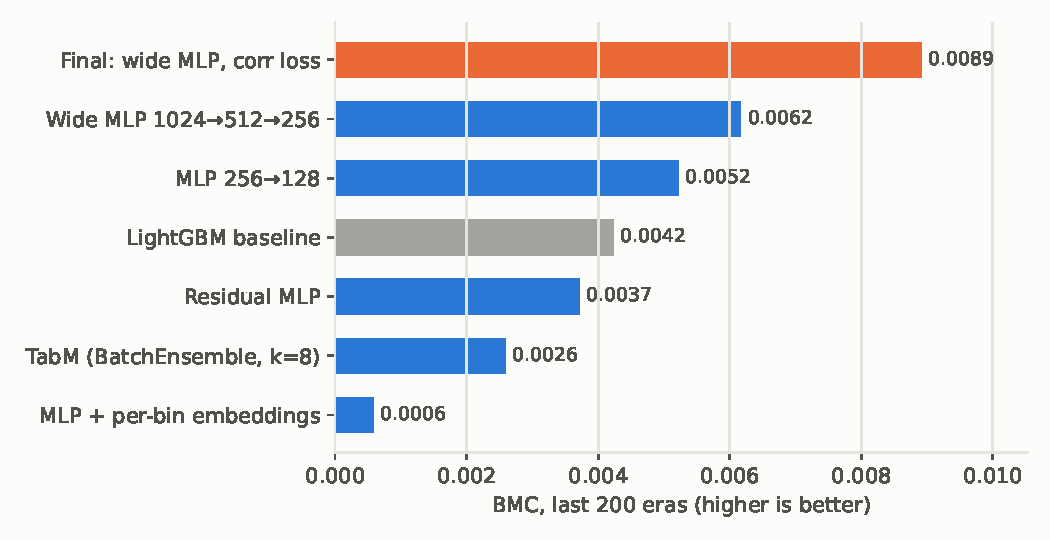
\includegraphics[width=0.85\linewidth]{figures/fig1_architectures.pdf}
\caption{\bmc{} over the last 200 OOF eras. Blue bars share the untuned round-1 recipe; gray is
the LightGBM baseline; orange is the final tuned model (correlation loss, learning rate
$2\times10^{-3}$, six epochs, three-seed average).}
\label{fig:arch}
\end{figure}

\subsection{Training amount governs contribution}

Training directly on per-era correlation lowers the benchmark correlation of predictions far
more than MSE does, but at 20 epochs it overfits badly: training-era correlation reached 0.24
against 0.018 out of fold. More dropout and weight decay, or an added MSE term, did not fix
this as well as simply training less.

Figure~\ref{fig:training} shows the mechanism. As the network trains, its predictions drift
steadily away from the benchmark (panel b), which raises \bmc{}, while raw correlation holds
roughly flat and then falls. \bmc{} therefore peaks just before raw correlation collapses
(panel a). Every knob that changes the amount of training lands on this curve: the optimal
epoch count moves from 8 to 6 when the learning rate doubles; a learning rate of
$5\times10^{-4}$ under-trains while $3\times10^{-3}$ over-trains; eight eras per batch halves the
number of updates and under-trains; and extra dropout or input dropout at the optimal length
behaves like less training, pulling predictions back towards the benchmark. Across all scout
runs, \bmc{} rises as benchmark correlation falls until raw signal is lost
(Figure~\ref{fig:tradeoff}).

\begin{figure}[t]
\centering
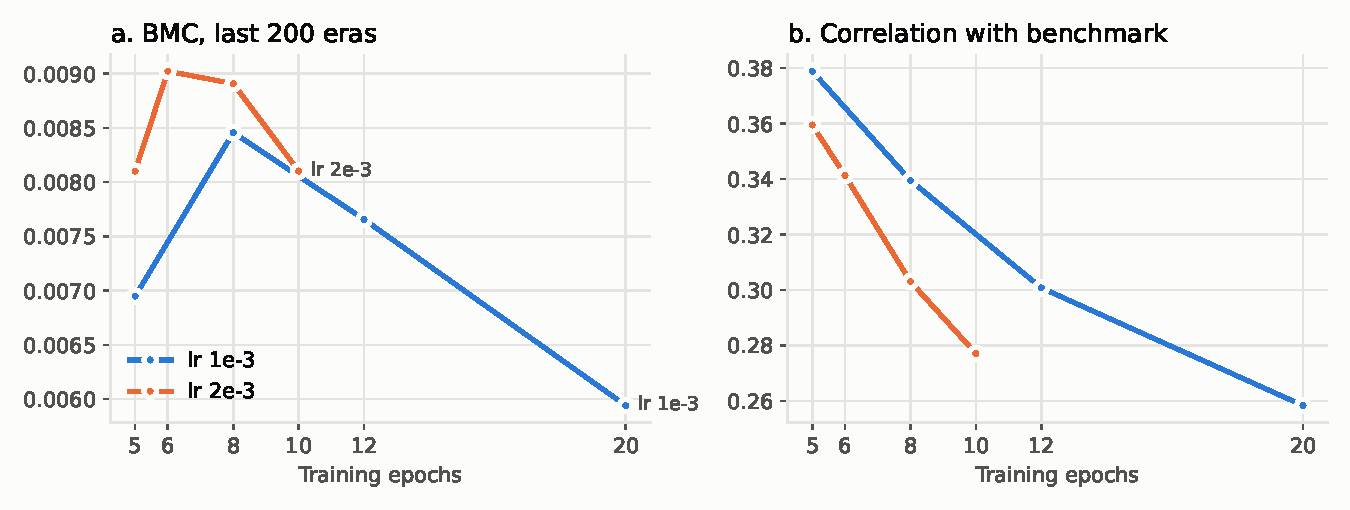
\includegraphics[width=\linewidth]{figures/fig2_training_amount.pdf}
\caption{Correlation-loss MLP (256--128), single seeds. (a) \bmc{} peaks at a training length
that depends on the learning rate. (b) Correlation with the benchmark falls the longer the
network trains. The point at learning rate $2\times10^{-3}$ and eight epochs is a lucky seed;
its three-seed average is 0.0083.}
\label{fig:training}
\end{figure}

\begin{figure}[t]
\centering
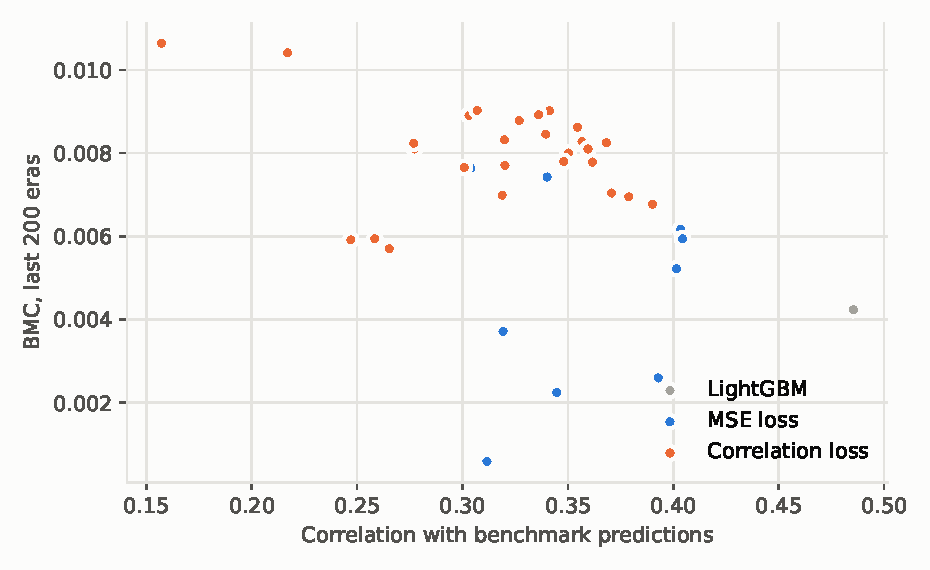
\includegraphics[width=0.72\linewidth]{figures/fig3_tradeoff.pdf}
\caption{All scout runs: correlation with the benchmark against \bmc{}. Lower benchmark
correlation buys contribution until raw signal collapses.}
\label{fig:tradeoff}
\end{figure}

\subsection{Seed noise and the confirmed winner}

Single-seed results vary by up to $\pm0.0006$ \bmc{}: one run at learning rate
$2\times10^{-3}$ scored 0.0089, but its three-seed average was 0.0083. We therefore judged
finalists on three-seed averages (Table~\ref{tab:final}). The wide and narrow winners'
predictions correlate 0.96, so averaging them adds nothing. Width helps only once training is
short enough to stop the network from memorizing. Figure~\ref{fig:cum} shows that the winner's
advantage accumulates steadily across eras rather than coming from a few outliers.

\begin{table}[t]
\centering\small
\begin{tabular}{p{5.4cm}ccccc}
\toprule
Model (scout data, 3 seeds) & corr & \bmc{} & \bmc{} last 200 & Sharpe & w/ bench. \\
\midrule
\textbf{Wide 1024--512--256, corr loss, lr 2e-3, 6 ep.} & 0.0260 & \textbf{0.0088} & \textbf{0.0089} & 0.71 & 0.336 \\
Narrow 256--128, corr loss, lr 2e-3, 6 ep. & 0.0262 & 0.0085 & 0.0086 & 0.71 & 0.355 \\
Narrow 256--128, corr loss, lr 1e-3, 8 ep. & 0.0261 & 0.0082 & 0.0083 & 0.68 & 0.357 \\
Rank average of wide and narrow & 0.0263 & 0.0087 & 0.0088 & 0.71 & -- \\
\bottomrule
\end{tabular}
\caption{Seed-averaged finalists on scout data.}
\label{tab:final}
\end{table}

\begin{figure}[t]
\centering
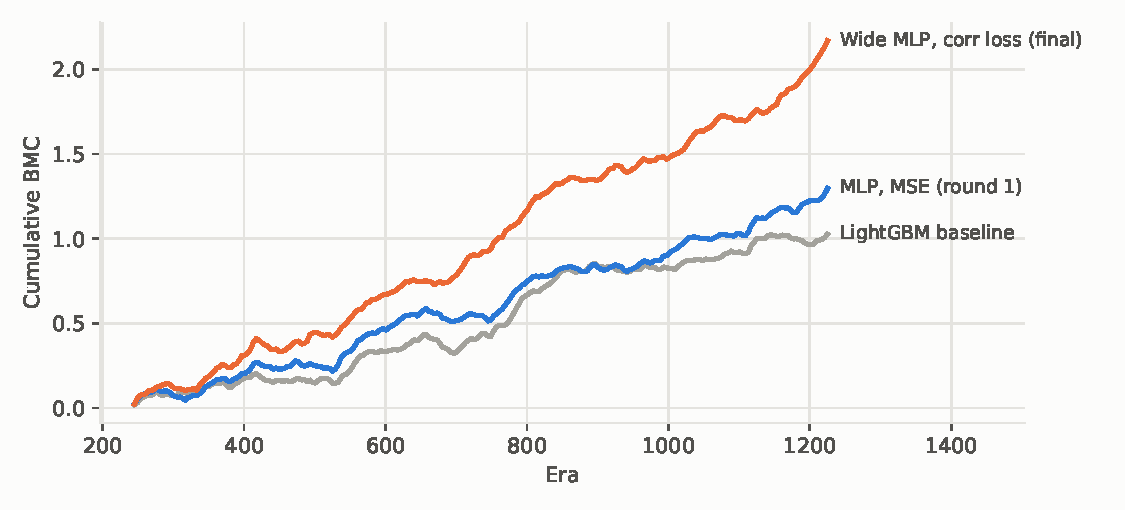
\includegraphics[width=0.9\linewidth]{figures/fig4_cumulative_bmc.pdf}
\caption{Cumulative per-era \bmc{} on the same 246 scout OOF eras.}
\label{fig:cum}
\end{figure}

\subsection{Confirmation on unseen eras}

We retrained the finalists on the scale data: 613 eras never used during the search, with
twice the training rows per fold (Table~\ref{tab:scale}). Run unchanged, the six-epoch winner
dropped to 0.0056, with exactly the signature of over-training seen in
Figure~\ref{fig:training}: lower raw correlation and lower benchmark correlation (0.28 against
0.34 on scout data). With twice the rows per epoch, six epochs means twice as many optimizer
steps. Cutting to four epochs recovers \bmc{}~0.0082 and returns benchmark correlation to its
scout level (0.33), on data the search never touched. The optimal training amount is
therefore a fixed number of optimizer steps, not epochs, consistent with the continuous-time
view in which stopping time sets the effective regularization \citep{ali2019continuous}.

\begin{table}[t]
\centering\small
\begin{tabular}{lcccc}
\toprule
Model (3 seeds) & corr & \bmc{} & \bmc{} last 200 & corr w/ benchmark \\
\midrule
Wide, 6 epochs, scout data (reference) & 0.0260 & 0.0088 & 0.0089 & 0.336 \\
Wide, 4 epochs, scale data & 0.0237 & 0.0074 & \textbf{0.0082} & 0.330 \\
Narrow, 6 epochs, scale data & 0.0220 & 0.0068 & 0.0067 & 0.308 \\
Wide, 6 epochs, scale data & 0.0206 & 0.0065 & 0.0056 & 0.283 \\
\bottomrule
\end{tabular}
\caption{Confirmation on 613 eras disjoint from the search. The last 200 eras of the scale
data are more recent than those of the scout data, so absolute levels are not directly
comparable.}
\label{tab:scale}
\end{table}

\section{Discussion}

\paragraph{Why does less capacity win?} Numerai's per-era signal is weak, with correlations
around 0.02, so spare capacity is spent fitting era-specific noise. The architectures that lost
all add capacity or flexibility; the winning changes all limit how far the network moves from
its initialization. This mirrors the shallow-network result for U.S.\ equities
\citep{gu2020empirical} and the strength of regularized plain MLPs on tabular data
\citep{kadra2021well}.

\paragraph{Why does a correlation loss help \bmc{}?} Squared error rewards predicting the
target's overall level and spread, which a tree benchmark already does well. A per-era Pearson
loss rewards only within-era ranking, the quantity Numerai scores, and in practice yields
predictions far less similar to the benchmark's.

\paragraph{A practical recipe.} For a new target or feature set, tune the amount of training
first, in optimizer steps, and pick the \bmc{} peak before adding architecture. When the
training set grows, scale the epoch count down so the number of steps stays at the optimum.

\paragraph{Limitations.} We used the \texttt{medium} feature set only; the 3,555-feature set did
not fit in memory. Since Numerai's round 1343 the official \bmc{} uses the 60-day Ender target
and a stake-weighted ensemble of benchmark models \citep{numerai_scoring}, so our 20-day,
single-benchmark \bmc{} is a proxy for the payout metric. Finalists were averaged over three
seeds, so differences below about 0.0003 should be read as ties. Thirty-five configurations
were tried on the same folds; a deflated Sharpe ratio \citep{bailey2014deflated} would temper
the best scout result, which is one reason we confirmed on disjoint eras. No live-tournament
results are included yet.

\section{Conclusion}

On Numerai's 20-day Ender target the best neural network is not an exotic one. A plain
three-layer MLP with a per-era correlation loss, trained briefly, doubles the LightGBM
baseline's benchmark contribution. Architecture mattered less than the amount of training,
which trades raw signal for uniqueness along a single curve, and that amount is best fixed in
optimizer steps. Next steps follow directly from the literature: interpolating trained weights
towards their initialization as a continuous training-amount dial \citep{ali2019continuous},
penalizing correlation with the benchmark during training, training on the 60-day target that
Numerai now pays on, and a quasi-Monte Carlo search over the learning-rate and step-count
interaction \citep{bousquet2017critical}.

\paragraph{Reproducibility.} Code, configurations, figures and this paper are in
\url{https://github.com/VolodymyrLinuxovich/example-scripts}, branch \path{nn-arch-ender20},
directory \path{numerai/agents/experiments/nn_arch_ender20}.

\bibliographystyle{plainnat}
\bibliography{references}

\appendix
\section{Full experiment log}
Every configuration that ran, by round. Single seeds unless the configuration says otherwise; bold marks each round's best \bmc{} over the last 200 eras.

\subsection*{Baselines}
\begin{center}\scriptsize\begin{tabular}{p{3.2cm}p{6.0cm}cccc}\toprule
Run & Configuration & corr & \bmc{} & last 200 & w/ bench. \\\midrule
\path{r0_baseline_small_lgbm} & LightGBM, 2,000 trees & 0.0277 & 0.0042 & \textbf{0.0042} & 0.485 \\
\path{r0_smoke_mlp} & MLP 256--128 $\cdot$ MSE $\cdot$ 1 ep $\cdot$ lr 0.001 & 0.0188 & 0.0024 & 0.0022 & 0.345 \\
\bottomrule\end{tabular}\end{center}

\subsection*{Round 1 $\cdot$ architecture}
\begin{center}\scriptsize\begin{tabular}{p{3.2cm}p{6.0cm}cccc}\toprule
Run & Configuration & corr & \bmc{} & last 200 & w/ bench. \\\midrule
\path{r1_mlp_wide_mse} & MLP 1024--512--256 $\cdot$ MSE $\cdot$ 4 ep $\cdot$ lr 0.001 $\cdot$ drop 0.2 & 0.0259 & 0.0061 & \textbf{0.0062} & 0.404 \\
\path{r1_mlp_corr} & MLP 256--128 $\cdot$ corr loss $\cdot$ 20 ep $\cdot$ lr 0.001 & 0.0184 & 0.0055 & 0.0059 & 0.258 \\
\path{r1_mlp_mse} & MLP 256--128 $\cdot$ MSE $\cdot$ 4 ep $\cdot$ lr 0.001 & 0.0249 & 0.0053 & 0.0052 & 0.402 \\
\path{r1_resmlp_mse} & Residual MLP w256 $\cdot$ MSE $\cdot$ 4 ep $\cdot$ lr 0.001 & 0.0187 & 0.0036 & 0.0037 & 0.319 \\
\path{r1_tabm_mse} & TabM 256--256 $\cdot$ MSE $\cdot$ 4 ep $\cdot$ lr 0.001 & 0.0213 & 0.0026 & 0.0026 & 0.393 \\
\path{r1_mlp_embed_mse} & MLP 256--128 $\cdot$ MSE $\cdot$ 4 ep $\cdot$ lr 0.001 $\cdot$ embeddings & 0.0157 & 0.0012 & 0.0006 & 0.312 \\
\bottomrule\end{tabular}\end{center}

\subsection*{Round 2 $\cdot$ training length}
\begin{center}\scriptsize\begin{tabular}{p{3.2cm}p{6.0cm}cccc}\toprule
Run & Configuration & corr & \bmc{} & last 200 & w/ bench. \\\midrule
\path{r2_corr_ep8} & MLP 256--128 $\cdot$ corr loss $\cdot$ 8 ep $\cdot$ lr 0.001 & 0.0253 & 0.0083 & \textbf{0.0085} & 0.340 \\
\path{r2_corr_epb1} & MLP 256--128 $\cdot$ corr loss $\cdot$ 5 ep $\cdot$ lr 0.001 $\cdot$ 1 era/batch & 0.0254 & 0.0078 & 0.0080 & 0.350 \\
\path{r2_wide_ep8} & MLP 1024--512--256 $\cdot$ MSE $\cdot$ 8 ep $\cdot$ lr 0.001 $\cdot$ drop 0.2 & 0.0229 & 0.0073 & 0.0076 & 0.304 \\
\path{r2_mse_ep8} & MLP 256--128 $\cdot$ MSE $\cdot$ 8 ep $\cdot$ lr 0.001 & 0.0244 & 0.0071 & 0.0074 & 0.340 \\
\path{r2_corr_reg} & MLP 256--128 $\cdot$ corr loss $\cdot$ 20 ep $\cdot$ lr 0.001 $\cdot$ drop 0.3 $\cdot$ wd 0.001 & 0.0230 & 0.0068 & 0.0070 & 0.319 \\
\path{r2_wider_mse} & MLP 2048--1024--512 $\cdot$ MSE $\cdot$ 4 ep $\cdot$ lr 0.001 $\cdot$ drop 0.3 & 0.0255 & 0.0057 & 0.0059 & 0.404 \\
\path{r2_wide_corr} & MLP 1024--512--256 $\cdot$ corr loss $\cdot$ 20 ep $\cdot$ lr 0.001 $\cdot$ drop 0.2 & 0.0183 & 0.0059 & 0.0059 & 0.247 \\
\path{r2_corr_mse} & MLP 256--128 $\cdot$ corr+MSE $\cdot$ 20 ep $\cdot$ lr 0.001 & 0.0184 & 0.0052 & 0.0057 & 0.265 \\
\bottomrule\end{tabular}\end{center}

\subsection*{Round 3 $\cdot$ refine}
\begin{center}\scriptsize\begin{tabular}{p{3.2cm}p{6.0cm}cccc}\toprule
Run & Configuration & corr & \bmc{} & last 200 & w/ bench. \\\midrule
\path{r3_corr_ep8_seeds3} & MLP 256--128 $\cdot$ corr loss $\cdot$ 8 ep $\cdot$ lr 0.001 $\cdot$ 3 seeds & 0.0261 & 0.0082 & \textbf{0.0083} & 0.357 \\
\path{r3_wide_corr_ep6} & MLP 1024--512--256 $\cdot$ corr loss $\cdot$ 6 ep $\cdot$ lr 0.001 $\cdot$ drop 0.2 & 0.0261 & 0.0079 & 0.0077 & 0.360 \\
\path{r3_corr_ep12} & MLP 256--128 $\cdot$ corr loss $\cdot$ 12 ep $\cdot$ lr 0.001 & 0.0225 & 0.0073 & 0.0077 & 0.301 \\
\path{r3_corr_ep5} & MLP 256--128 $\cdot$ corr loss $\cdot$ 5 ep $\cdot$ lr 0.001 & 0.0253 & 0.0067 & 0.0069 & 0.379 \\
\path{r3_corr_ep8_drop03} & MLP 256--128 $\cdot$ corr loss $\cdot$ 8 ep $\cdot$ lr 0.001 $\cdot$ drop 0.3 & 0.0260 & 0.0067 & 0.0068 & 0.390 \\
\bottomrule\end{tabular}\end{center}

\subsection*{Round 4 $\cdot$ new knobs}
\begin{center}\scriptsize\begin{tabular}{p{3.2cm}p{6.0cm}cccc}\toprule
Run & Configuration & corr & \bmc{} & last 200 & w/ bench. \\\midrule
\path{r4_lr2e3} & MLP 256--128 $\cdot$ corr loss $\cdot$ 8 ep $\cdot$ lr 0.002 & 0.0237 & 0.0084 & \textbf{0.0089} & 0.303 \\
\path{r4_indrop01} & MLP 256--128 $\cdot$ corr loss $\cdot$ 8 ep $\cdot$ lr 0.001 $\cdot$ in-drop 0.1 & 0.0263 & 0.0079 & 0.0083 & 0.368 \\
\path{r4_epb8} & MLP 256--128 $\cdot$ corr loss $\cdot$ 8 ep $\cdot$ lr 0.001 $\cdot$ 8 era/batch & 0.0250 & 0.0072 & 0.0078 & 0.362 \\
\path{r4_deep} & MLP 512--256--128 $\cdot$ corr loss $\cdot$ 8 ep $\cdot$ lr 0.001 & 0.0241 & 0.0076 & 0.0077 & 0.320 \\
\path{r4_lr5e4} & MLP 256--128 $\cdot$ corr loss $\cdot$ 8 ep $\cdot$ lr 0.0005 & 0.0252 & 0.0068 & 0.0070 & 0.371 \\
\bottomrule\end{tabular}\end{center}

\subsection*{Round 5 $\cdot$ lr 2e-3}
\begin{center}\scriptsize\begin{tabular}{p{3.2cm}p{6.0cm}cccc}\toprule
Run & Configuration & corr & \bmc{} & last 200 & w/ bench. \\\midrule
\path{r5_lr2e3_ep6} & MLP 256--128 $\cdot$ corr loss $\cdot$ 6 ep $\cdot$ lr 0.002 & 0.0257 & 0.0087 & \textbf{0.0090} & 0.341 \\
\path{r5_wide_lr2e3_ep6} & MLP 1024--512--256 $\cdot$ corr loss $\cdot$ 6 ep $\cdot$ lr 0.002 $\cdot$ drop 0.2 & 0.0256 & 0.0088 & 0.0088 & 0.327 \\
\path{r5_lr2e3_seeds3} & MLP 256--128 $\cdot$ corr loss $\cdot$ 8 ep $\cdot$ lr 0.002 $\cdot$ 3 seeds & 0.0242 & 0.0080 & 0.0083 & 0.320 \\
\path{r5_lr3e3} & MLP 256--128 $\cdot$ corr loss $\cdot$ 8 ep $\cdot$ lr 0.003 & 0.0217 & 0.0078 & 0.0082 & 0.277 \\
\path{r5_lr2e3_ep10} & MLP 256--128 $\cdot$ corr loss $\cdot$ 10 ep $\cdot$ lr 0.002 & 0.0216 & 0.0075 & 0.0081 & 0.277 \\
\bottomrule\end{tabular}\end{center}

\subsection*{Round 6 $\cdot$ seed check}
\begin{center}\scriptsize\begin{tabular}{p{3.2cm}p{6.0cm}cccc}\toprule
Run & Configuration & corr & \bmc{} & last 200 & w/ bench. \\\midrule
\path{r6_wide_lr2e3_ep6_seeds3} & MLP 1024--512--256 $\cdot$ corr loss $\cdot$ 6 ep $\cdot$ lr 0.002 $\cdot$ drop 0.2 $\cdot$ 3 seeds & 0.0260 & 0.0088 & \textbf{0.0089} & 0.336 \\
\path{r6_lr2e3_ep6_seeds3} & MLP 256--128 $\cdot$ corr loss $\cdot$ 6 ep $\cdot$ lr 0.002 $\cdot$ 3 seeds & 0.0262 & 0.0085 & 0.0086 & 0.355 \\
\path{r6_lr2e3_ep5} & MLP 256--128 $\cdot$ corr loss $\cdot$ 5 ep $\cdot$ lr 0.002 & 0.0258 & 0.0080 & 0.0081 & 0.360 \\
\path{r6_wide_lr2e3_ep5} & MLP 1024--512--256 $\cdot$ corr loss $\cdot$ 5 ep $\cdot$ lr 0.002 $\cdot$ drop 0.2 & 0.0257 & 0.0079 & 0.0078 & 0.348 \\
\bottomrule\end{tabular}\end{center}

\subsection*{Round 7 $\cdot$ literature ideas}
\begin{center}\scriptsize\begin{tabular}{p{3.2cm}p{6.0cm}cccc}\toprule
Run & Configuration & corr & \bmc{} & last 200 & w/ bench. \\\midrule
\path{r7_bench_pen1} & MLP 1024--512--256 $\cdot$ corr loss $\cdot$ 6 ep $\cdot$ lr 0.002 $\cdot$ drop 0.2 & 0.0188 & 0.0103 & \textbf{0.0106} & 0.157 \\
\path{r7_bench_pen03} & MLP 1024--512--256 $\cdot$ corr loss $\cdot$ 6 ep $\cdot$ lr 0.002 $\cdot$ drop 0.2 & 0.0216 & 0.0102 & 0.0104 & 0.217 \\
\path{r7_bmc_loss} & MLP 1024--512--256 $\cdot$ corr loss $\cdot$ 6 ep $\cdot$ lr 0.002 $\cdot$ drop 0.2 & 0.0248 & 0.0090 & 0.0090 & 0.307 \\
\bottomrule\end{tabular}\end{center}

\subsection*{Scale $\cdot$ unseen eras}
\begin{center}\scriptsize\begin{tabular}{p{3.2cm}p{6.0cm}cccc}\toprule
Run & Configuration & corr & \bmc{} & last 200 & w/ bench. \\\midrule
\path{s1_wide_ep3_seeds3} & MLP 1024--512--256 $\cdot$ corr loss $\cdot$ 3 ep $\cdot$ lr 0.002 $\cdot$ drop 0.2 $\cdot$ 3 seeds & 0.0262 & 0.0083 & \textbf{0.0095} & 0.365 \\
\path{s1_wide_ep4_seeds3} & MLP 1024--512--256 $\cdot$ corr loss $\cdot$ 4 ep $\cdot$ lr 0.002 $\cdot$ drop 0.2 $\cdot$ 3 seeds & 0.0237 & 0.0074 & 0.0082 & 0.330 \\
\path{s1_narrow_ep6_seeds3} & MLP 256--128 $\cdot$ corr loss $\cdot$ 6 ep $\cdot$ lr 0.002 $\cdot$ 3 seeds & 0.0220 & 0.0068 & 0.0067 & 0.308 \\
\path{s1_wide_ep6_seeds3} & MLP 1024--512--256 $\cdot$ corr loss $\cdot$ 6 ep $\cdot$ lr 0.002 $\cdot$ drop 0.2 $\cdot$ 3 seeds & 0.0206 & 0.0065 & 0.0056 & 0.283 \\
\path{s1_wide_mse_ep8} & MLP 1024--512--256 $\cdot$ MSE $\cdot$ 8 ep $\cdot$ lr 0.001 $\cdot$ drop 0.2 & 0.0164 & 0.0049 & 0.0027 & 0.233 \\
\bottomrule\end{tabular}\end{center}


\end{document}
